\documentclass[12pt,letterpaper]{article}

\usepackage[top=2cm,right=2cm,bottom=2cm,left=2cm,nohead,nofoot]{geometry}

\usepackage{amsmath}
\usepackage{graphicx}
\usepackage{indentfirst}
\usepackage{url}
\usepackage{mdwlist}
\usepackage[compact]{titlesec}
\usepackage[T1]{fontenc}
\usepackage{palatino}
\usepackage[brazil]{babel}
\usepackage[utf8]{inputenc}
\usepackage{enumerate}

\pagestyle{empty}
\setcounter{secnumdepth}{5}
\renewcommand{\thefootnote}{\Roman{footnote}}

\makeatletter
\def\thickhrulefill{\leavevmode \leaders \hrule height 1pt\hfill \kern \z@}
\renewcommand{\maketitle}{
	\begingroup
		\parindent \z@
		\begin{center}
			{\normalsize \@author\par}%
			\thickhrulefill\par
			{\small\raggedleft \@date\par}%
			{\Large\raggedright \@title\par}%
		\end{center}%
	\endgroup
}
\makeatother

\title{F 429: Experimento II}
\author{033910 Leandro Mendes | 104198 Thiago Verratti | 118451 Rafael Mendes | 121096 Leonardo Sorensen}
\begin{document}
\maketitle
\tableofcontents
\listoffigures
\listoftables
\newpage
\section{Introdução}
Este experimento propõe-se a estudar as experimentalmente e analizar as formas de onda dos circuitos integrador e
diferenciador. Neste caso, são do tipo RC e compostos por uma fonte, um resistor e um
capacitor ligados em série.\\
Analisamos também transientes em circuito ressonante série RLC. Os transientes podem ser estudados no laboratório excitando o circuito com uma onda quadrada de período muito maior que a constante de tempo do circuito.
\section{Instrumentos e Componentes}
Os instrumentos e componentes utilizados estão listados abaixo com seus respectivos valores nominais.
\begin{itemize}
\item{Gerador de Funções Tektronix CFG 253.} 
\item{Osciloscópio digital Tektronix TDS1000.}
\item{Resistências nominais de 47$\Omega$ e 150$\Omega$.}
\item{Resistência de décadas (10$\Omega$ a 10K$\Omega$).}
\item{Capacitor de 0.22$\mu$F.}
\item{Indutor de 50mH.}
\end{itemize}
\subsection{Medidas}
\subsubsection{Impedância interna do gerador} \label{itm:rger} Para determinar a impedância interna do gerador de funções, começamos com a aproximação de que esta é puramente resistiva e independe da frequência, modo de onda ou corrente que fornece. Feita essa hipótese, podemos encontrar a resistência interna $R_G$ do gerador montando o circuito como na figura abaixo. 
\begin{figure}[!htb]
  \centering
  \label{imgger}
  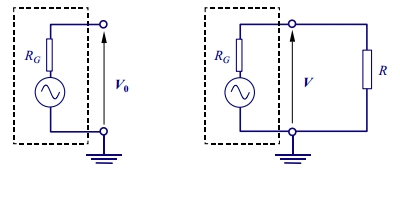
\includegraphics[scale=0.5]{impger.jpg}
  \caption{Circuito representativo para medida da resistência interna do gerador}
\end{figure}
Primeiro medimos a tensão de saída do gerador de funções conectando-o diretamente ao osciloscópio. Após medir o pico $V_0$, colocamos um resistor em paralelo ao circuito, e obtemos um valor para V. Com essas medidas podemos encontrar um valor para $R_G$, sabendo que temos um divisor de tensão e juntando a Lei de Ohm \footnote{\boxed{V = R\cdot I}}. Logo, $R_G = R \cdot (\frac{V_0}{V}-1)$ e $\Delta{R_G} = R_G \cdot \sqrt{(\frac{\Delta(\frac{V_0}{V})}{\frac{V_0}{V}-1})^2 + (\frac{\Delta{R}}{R})^2}$, onde $\Delta{\frac{V_0}{V}} = \frac{V_0}{V} \cdot \sqrt{(\frac{\Delta{V_0}}{V_0})^2 + (\frac{\Delta{V}}{V})^2}$.\\ Portanto, para \boxed{V_0 = 24,8V}\footnote{Escala: 5V}, \boxed{V = 12,2V}\footnote{Escala: 2V} e \boxed{R_{47} = 47,8\Omega , \Delta{R_{47}}=0,6\Omega}\footnote{Dado obtido no experimento I}, temos: \boxed{\Delta{V_0}=0,9940V, \Delta{V}=0,4660V}, resultando em \boxed{\frac{V_0}{V}=2,0328\frac{V}{V}, \Delta{\frac{V_0}{V}}=0,1125\frac{V}{V}} e \boxed{R_G = 49,3672\Omega \pm 5,4154\Omega}.
\subsubsection{Indutor}\label{itm:indutor} No experimento I, calculamos o valor do indutor utilizado nos experimentos. O resultado foi, \boxed{L = 47,0311mH \pm 4,0174mH}.
\subsubsection{Resistência em série do indutor ($R_L$)} \label{itm:rindutor}  O cálculo de $R_L$ foi apresentado no relatório I, resultando em \boxed{R_L = 46,3\Omega \pm 0,6\Omega}.
\subsubsection{Capacitor} \label{itm:capacitor} No experimento anterior obtivemos \boxed{C = 0,2236\mu F \pm 0,0191\mu F}.
\subsubsection{Resistor de 47$\Omega$}\label{itm:r47} \boxed{R_{47} = 47,8\Omega \pm 0,6\Omega}.
\subsubsection{Resistor de 150$\Omega$}\label{itm:r150} \boxed{R_{150} = 148\Omega \pm 2,5\Omega}.
\section{Circuito RC}
\subsubsection{Integrador}
Um circuito integrador é um componente eletrônico contendo elementos, como fonte de tensão[\ref{itm:rger}], resistor[\ref{itm:r150}] e capacitor[\ref{itm:capacitor}].
\begin{figure}[!htb]
  \centering
  \label{imgint}
  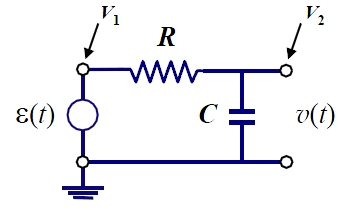
\includegraphics[scale=0.5]{integrador.jpg}
  \caption{Circuito integrador ou Filtro passa-baixa}
\end{figure}
\begin{enumerate}[I]
\item \textbf{Lei de Kirchoff}: Aplicando a lei de Kirchoff para malhas teremos: $\varepsilon(t) = R\cdot i(t) + v_c(t)$\footnote{Lembrando que \boxed{I_c(t) = C \cdot \frac{\mathrm d V(t)}{\mathrm d t}}}
\item \textbf{Integrador}: No cálculo acima obtemos: $v(t)\approx v_0(t) + \frac{1}{RC} \int_{t_0}^{t} \varepsilon(t)dt.$
\item \label{itm:passabaixa} \textbf{Passa-baixa}: A função de transferência de um passa-baixa\footnote{Sedra Smith, microeletronics circuits 5th edition , tabela 1.2: Resposta em frequência de redes STC} é dada por $T(s) = \frac{K}{1 + \frac{s}{w_0}}$.\\
  Sabe-se que $s = j \cdot w$, onde $w = 2\pi \cdot f$ e $\tau = \frac{1}{w_0}$\footnote{frequência 3-dB}.\\
Portanto, para um passa-baixa temos: $T(jw) = \frac{K}{1 + j(\frac{w}{w_0})}$ e a frequência de corte $f_c = \frac{1}{\tau \cdot 2\pi}$.
\subitem \label{itm:intdc} \textbf{Transmissão DC}: Em uma transmisao DC, ou seja, $f = 0Hz (w = 0)$, temos $T(jw) = K$.
\item \textbf{Metodologia}: Montamos o circuito conforme a figura acima, monitorando a $V_1$ e $V_2$ no osciloscópio, variando as formas de onda\footnote{quadrada, triângular e senoíde} e a frequência ( $\frac{f_c}{40}$ , $f_c$, $40f_c$ ). Modificamos, também, o nível DC entre -1V e +1V e observamos o efeito provocado.
\item \label{itm:intred} \textbf{Resultados e Discussões}: Dado em \ref{itm:passabaixa}, combinando com \ref{itm:capacitor} e \ref{itm:r150}, temos $f_c \approx 4,8881Hz$.
\begin{figure}[!htb]
  \centering
  \label{fd40int}
  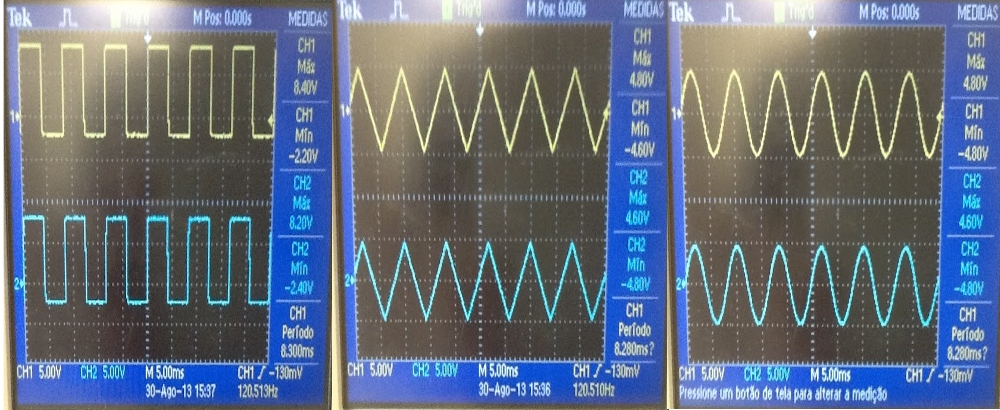
\includegraphics[scale=0.52]{img/fd40int.jpg}
  \caption{Circuito integrador $f_c \approx 120,51Hz$}
\end{figure}
\begin{figure}[!htb]
  \centering
  \label{fint}
  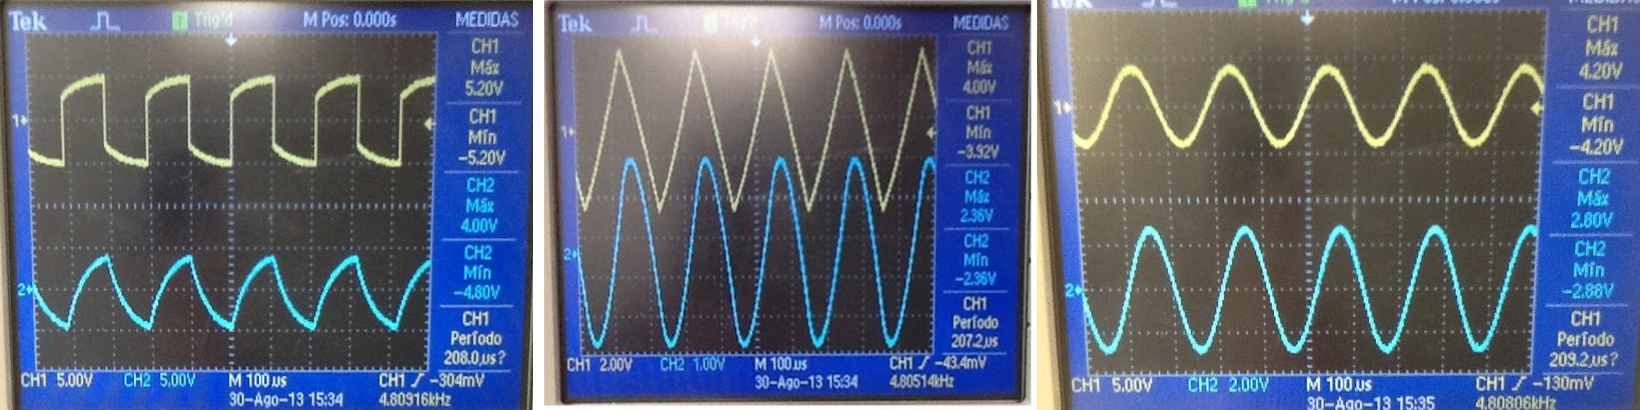
\includegraphics[scale=0.32]{img/fint.jpg}
  \caption{Circuito integrador $f_c$}
\end{figure}
\begin{figure}[!htb]
  \centering
  \label{f40int}
  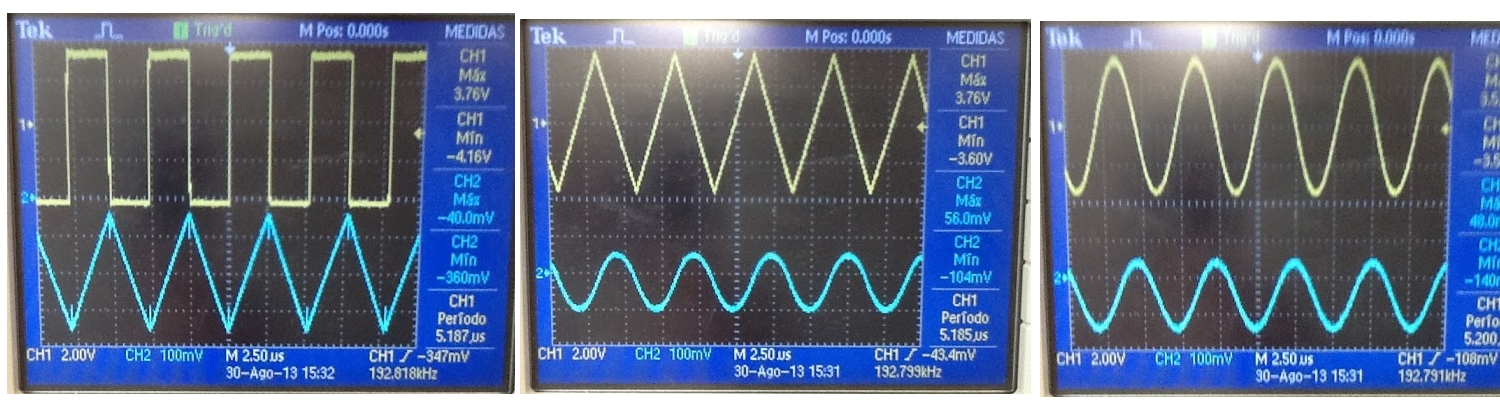
\includegraphics[scale=0.35]{img/f40int.jpg}
  \caption{Circuito integrador $f_c \approx 192,80kHz$}
\end{figure}
Para \ref{fd40int}, ou seja, frequências aquém de $f_c$, temos que $V_1 \approx V_2$ visto que o circuito é um passa-baixa[\ref{itm:passabaixa}]\footnote{Nota-se no diagrama de Bode do experimento I para um circuito RC}. Entretanto, para frequência próximas de $f_c$ observamos pequenas distorções em $V_2$ e para frequência muito além ($40f_c$) temos um integrador, visto que, a integral de uma constante é uma reta. \\
A variação do sinal DC resultou em uma descida/subida mais abrupta, já que teremos $T(jw) = K = 1, para f = 0$.
\end{enumerate}
\subsubsection{Diferenciador}
O circuito RC diferenciador assemelha-se ao integrador, apenas alteramos a configuração entre o resistor \ref{itm:r150} e o capacitor \ref{itm:capacitor}.
\begin{figure}[!htb]
  \centering
  \label{imgint}
  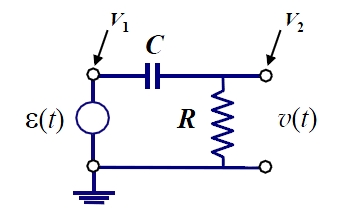
\includegraphics[scale=0.5]{diferenciador.jpg}
  \caption{Circuito diferenciador ou Filtro passa-alta}
\end{figure}
\begin{enumerate}[I]
\item \textbf{Lei de Kirchoff}: Aplicando a lei de Kirchoff para malhas teremos: $\varepsilon(t) = \frac{t}{C} + v(t)$.
\item \textbf{Diferenciador}: No cálculo acima obtemos: $v(t) \approx \frac{1}{RC}\frac{d\varepsilon(t)}{dt}$
\item \label{itm:passaalta} \textbf{Passa-alta}: A função de transferência de um passa-alta\footnote{Sedra Smith, microeletronics circuits 5th edition , tabela 1.2: Resposta em frequência de redes STC} é dada por $T(s) = \frac{Ks}{s + w_0}$.\\
  Sabe-se que $s = j \cdot w$, onde $w = 2\pi \cdot f$ e $\tau = \frac{1}{w_0}$\footnote{frequência 3-dB}.\\
Portanto, para um passa-alta temos: $T(jw) = \frac{K}{1 - j(\frac{w_0}{w})}$ e a frequência de corte $f_c = \frac{1}{\tau \cdot 2\pi}$.
\subitem \label{itm:intdc} \textbf{Transmissão DC}: Em uma transmisao DC, ou seja, $f = 0Hz (w = 0)$, temos $T(jw) = 0$.
\item \textbf{Metodologia}: Montamos o circuito conforme a figura acima, monitorando a $V_1$ e $V_2$ no osciloscópio, variando as formas de onda\footnote{quadrada, triângular e senoíde} e a frequência ( $\frac{f_c}{40}$ , $f_c$, $40f_c$ ). Modificamos, também, o nível DC entre -1V e +1V e observamos o efeito provocado.
\item \label{itm:intred} \textbf{Resultados e Discussões}: Dado para um filtro passa-alta \ref{itm:passaalta}, combinando com o capacitor \ref{itm:capacitor} e resistor \ref{itm:r150}, temos:
\begin{figure}[!htb]
  \centering
  \label{fd40d}
  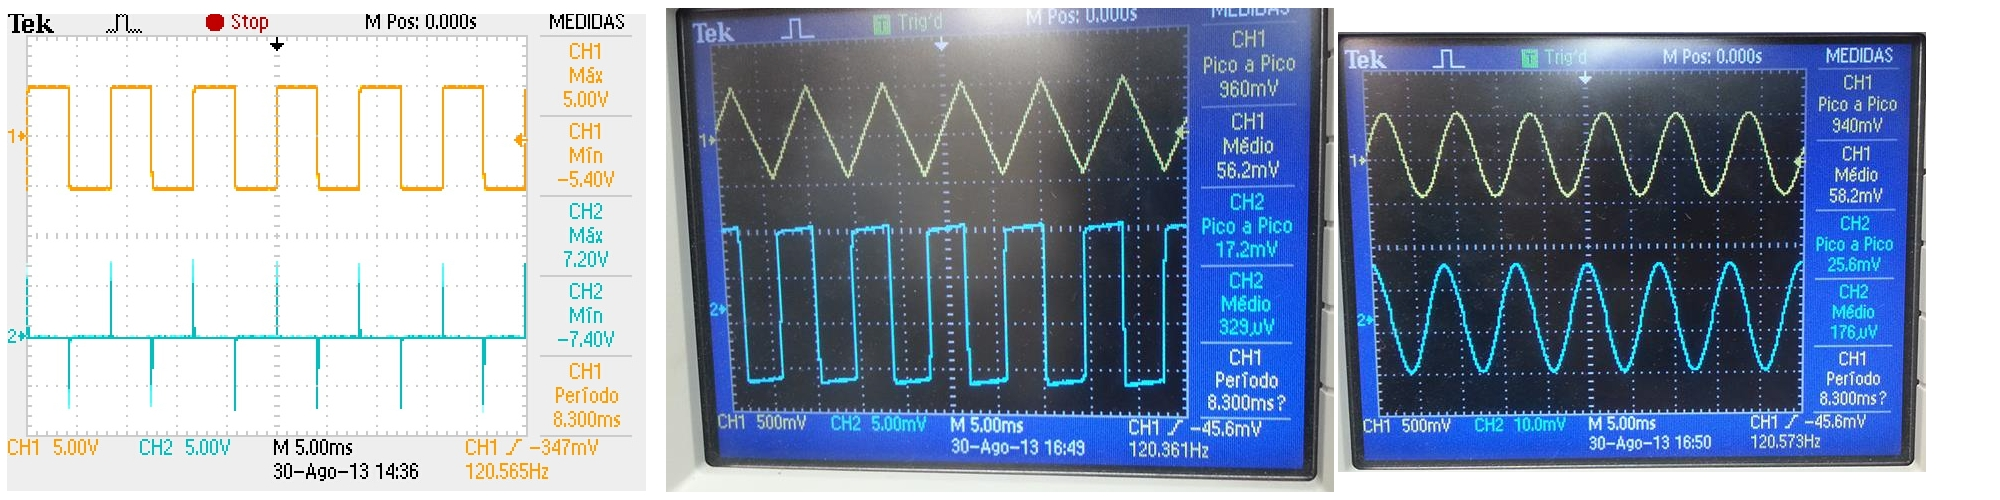
\includegraphics[scale=0.62]{img/fd40d.jpg}
  \caption{Circuito diferenciador $f_c \approx 120,51Hz$}
\end{figure}
\begin{figure}[!htb]
  \centering
  \label{fd}
  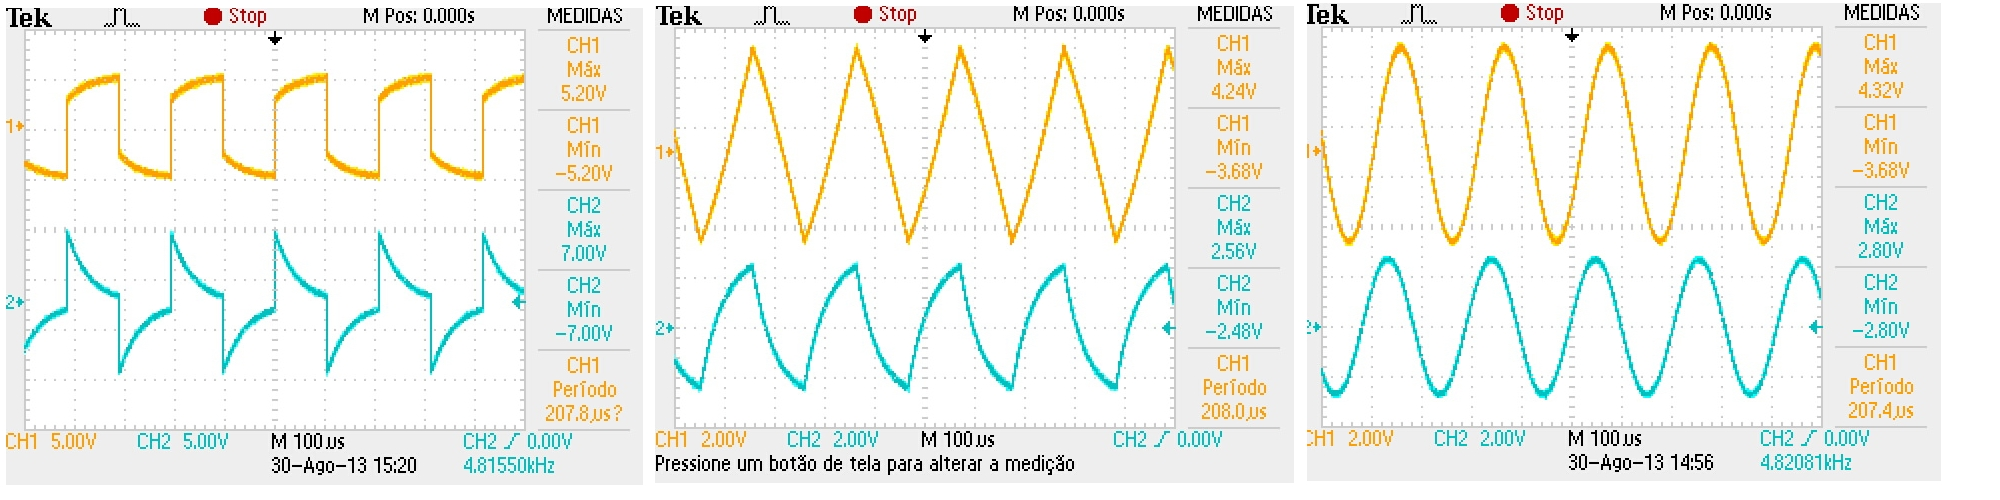
\includegraphics[scale=0.62]{img/fd.jpg}
  \caption{Circuito diferenciador $f_c$}
\end{figure}
\begin{figure}[!htb]
  \centering
  \label{f40d}
  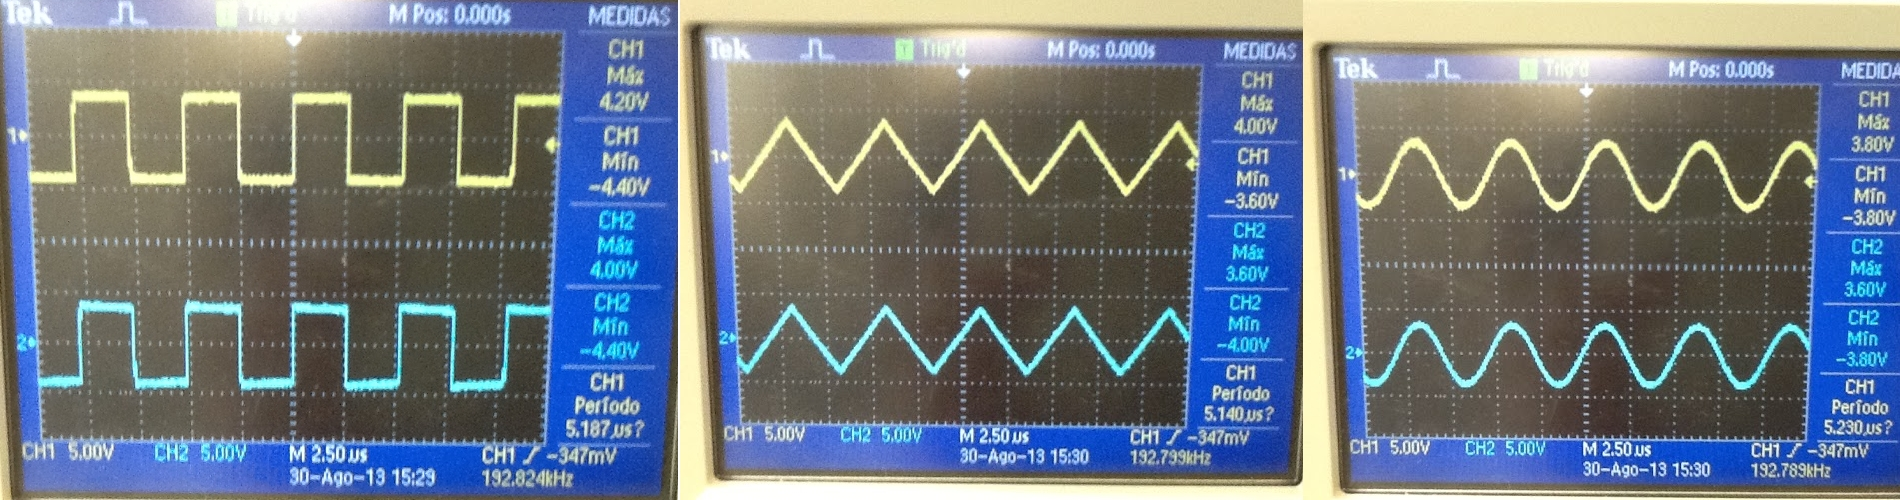
\includegraphics[scale=0.25]{img/f40d.jpg}
  \caption{Circuito diferenciador $f_c \approx 192,80kHz$}
\end{figure}
Para \ref{fd40d}, ou seja, frequências aquém de $f_c$, temos um circuito integrador, conforme observado na figura \ref{fd40d}, na qual para a onda triângular, fica claro que, a derivada de uma reta é uma constante. Já para frequência bem próxima a $f_c$ temos uma distorção na saída, e para $f >> f_c, ou seja, f \approx 40f_c$ temos $V_1 \approx V_2$, visto que temos um filtro passa-alta. 
A variação do sinal DC não modificou a saída $V_2$, uma vez que, o capacitor carrega-se rápidamente em tensão/corrente DC e, diferentemente de uma onda variável no tempo, o capacitor não se descarregará.
Observamos abaixo, a região de descontinuidade do diferenciador, isso acontece quando o mesmo está em baixas frequências, ou seja, atuando como um diferenciador.
\begin{figure}[!htb]
  \centering
  \label{decont}
  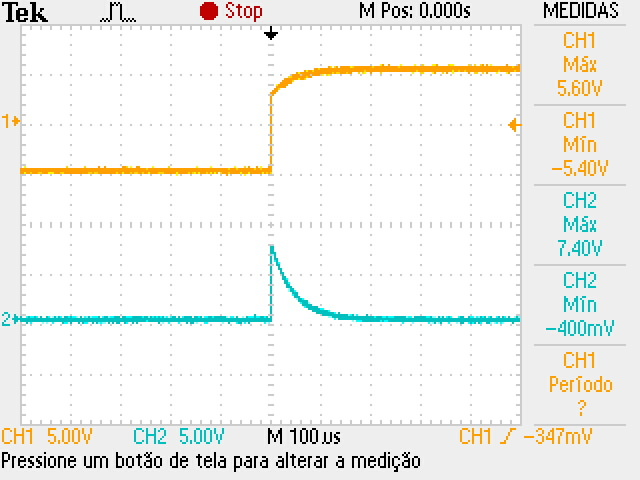
\includegraphics[scale=0.5]{img/descontinuidade.jpg}
  \caption{Circuito diferenciador descontinuidade}
\end{figure}
\end{enumerate}
\section{Circuito RLC}
Neste experimento, montamos um circuito RLC, de acordo com a figura abaixo. Onde $R_L$[\ref{itm:rindutor}] é a resistência inerente ao indutor, L[\ref{itm:indutor}] o indutor, C[\ref{itm:capacitor}] o capacitor e $R_D$ é a resistência de década. $R_g$ é a resistência interna do gerador.
\begin{figure}[!htb]
  \centering
  \label{imgrlc}
  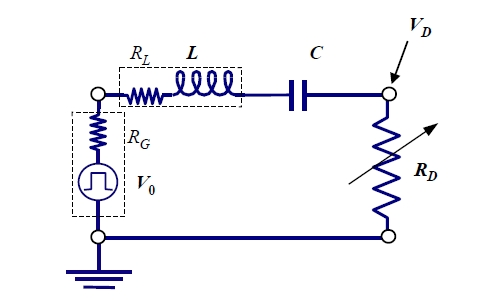
\includegraphics[scale=0.5]{img/rlc.jpg}
  \caption{Circuito RLC}
\end{figure}
A resistência interna do gerador foi determinada medindo a voltagem de circuito aberto e a voltagem quando conectado a um resistor de 47 ohms, já a RL foi medida com um multímetro. O valor da capacitância e da indutância foi determinada com o método da figura de Lissajous.\\
Com as medidas em mãos iniciamos nosso experimento com o procedimento descrito abaixo:
\begin{enumerate}[I]
\item O osciloscópio configurado para monitorar a voltagem no gerador e a corrente, ou seja no canal 2 está a resistência de décadas.
\item Ligamos o gerador de forma a alimentar o circuito com o formato de onda senoidal.
\item Determinamos a frequencia de ressonância - $f_0$ - pelo método de Lissajous.
\item Variamos a resistência de décadas para verificarmos que $f_0$ \textbf{NÃO} depende de $R_d$.
\item Após isso, aliementamos o circuito com ondas quadradas e ajustamos a frequência do gerador de forma a garantir que a corrente zera a casa semiciclo ( $ T < 10 \cdot \tau $), onde T é o periodo de onda e $\tau=\frac{2L}{R}$.
\item Variando a resistência de década pudemos observar a mudança dos regimes de amortecimento.
\end{enumerate}
\subsection{Teoria e Experimento}
Nesta parte, iremos tratar da teoria e ao mesmo tempo mostraremos os dados experiementais, de forma a melhor confrontar um com o outro.\\
Na presente parte do experimento analisamos os transientes não repetitivos em um circuito ressoante série ao ligarmos uma voltagem constante, que está indicada nas fotos e legendas. O gerador fornece uma forma de onda que vale 0 para $t < 0$ e uma constante $E_{pp}$, para t positivo, ou seja: $E(t) = E_{pp}\mu (t)$, sendo $\mu (t)$ uma função degrau, ou Heaviside\footnote{\url{http://www.scribd.com/doc/15995098/21/Transientes-no-circuito-ressonante-serie}}.\\
A equação de malha do circuito RLC série é: $ L \frac{d^2q}{dt^2} + R\frac{dq}{dt} +\frac{Q}{C} = E_{pp}\mu$ e o fator de mérito do circuito ressonante série, que caracteriza a acuidade da curva de ressonância dada pela equação: $ Q = \omega_0 \cdot \frac{L}{R} = \frac{\omega}{\Delta \omega}$, sendo $q = q(t)$ a carga instantânea no capacitor, e esta equação por ser uma diferencial de segundo grau depende de duas condições iniciais. Como na função degrau a voltagem é zero para todo $t < 0$, o capacitor não pode estar carregado e a corrente não estaria passado em $t = 0$. Portanto temos: $ q(t) = C E_{pp}[1 - e^{\frac{-t}{\tau}}(cos(\omega t) + \frac{1}{\omega \tau}sen(\omega t))]$. Assim obtemos a frequência natural de oscilação $\omega$. As oscilações são amortecidas exponencialmente com a constante de tempo $\tau$, como a figura abaixo mostra a resposta esperada do sub-amorteciemento:
\begin{figure}[!htb]
  \centering
  \label{subteo}
  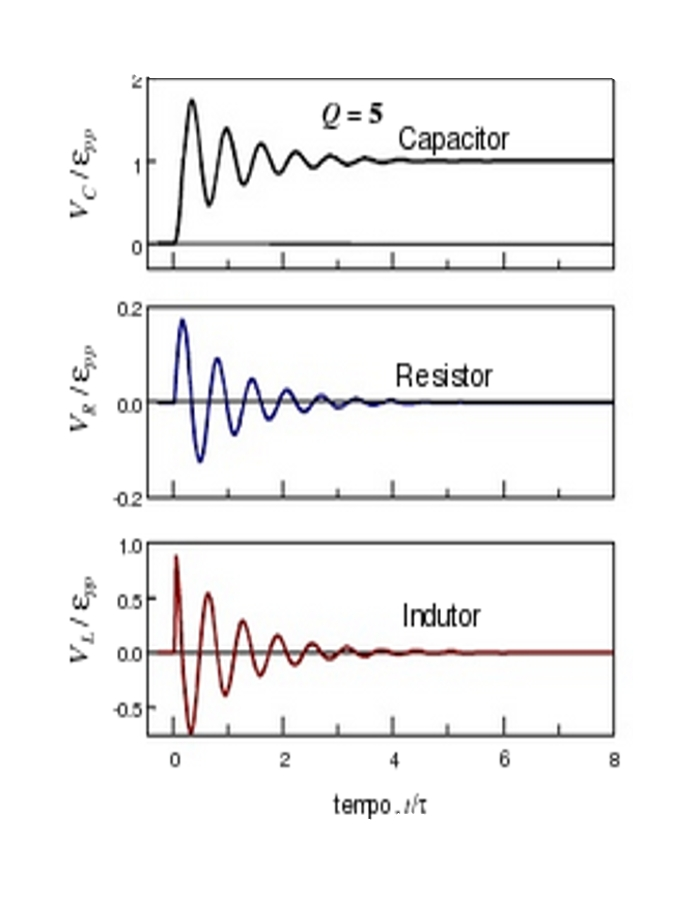
\includegraphics[scale=0.30]{img/subamortecido.jpg}
  \caption{Componentes em estado subamorticidos}
\end{figure}
E conforme podemos ver na figura seguinte, obtivemos os gráficos:
\begin{figure}[!htb]
  \centering
  \label{mysub}
  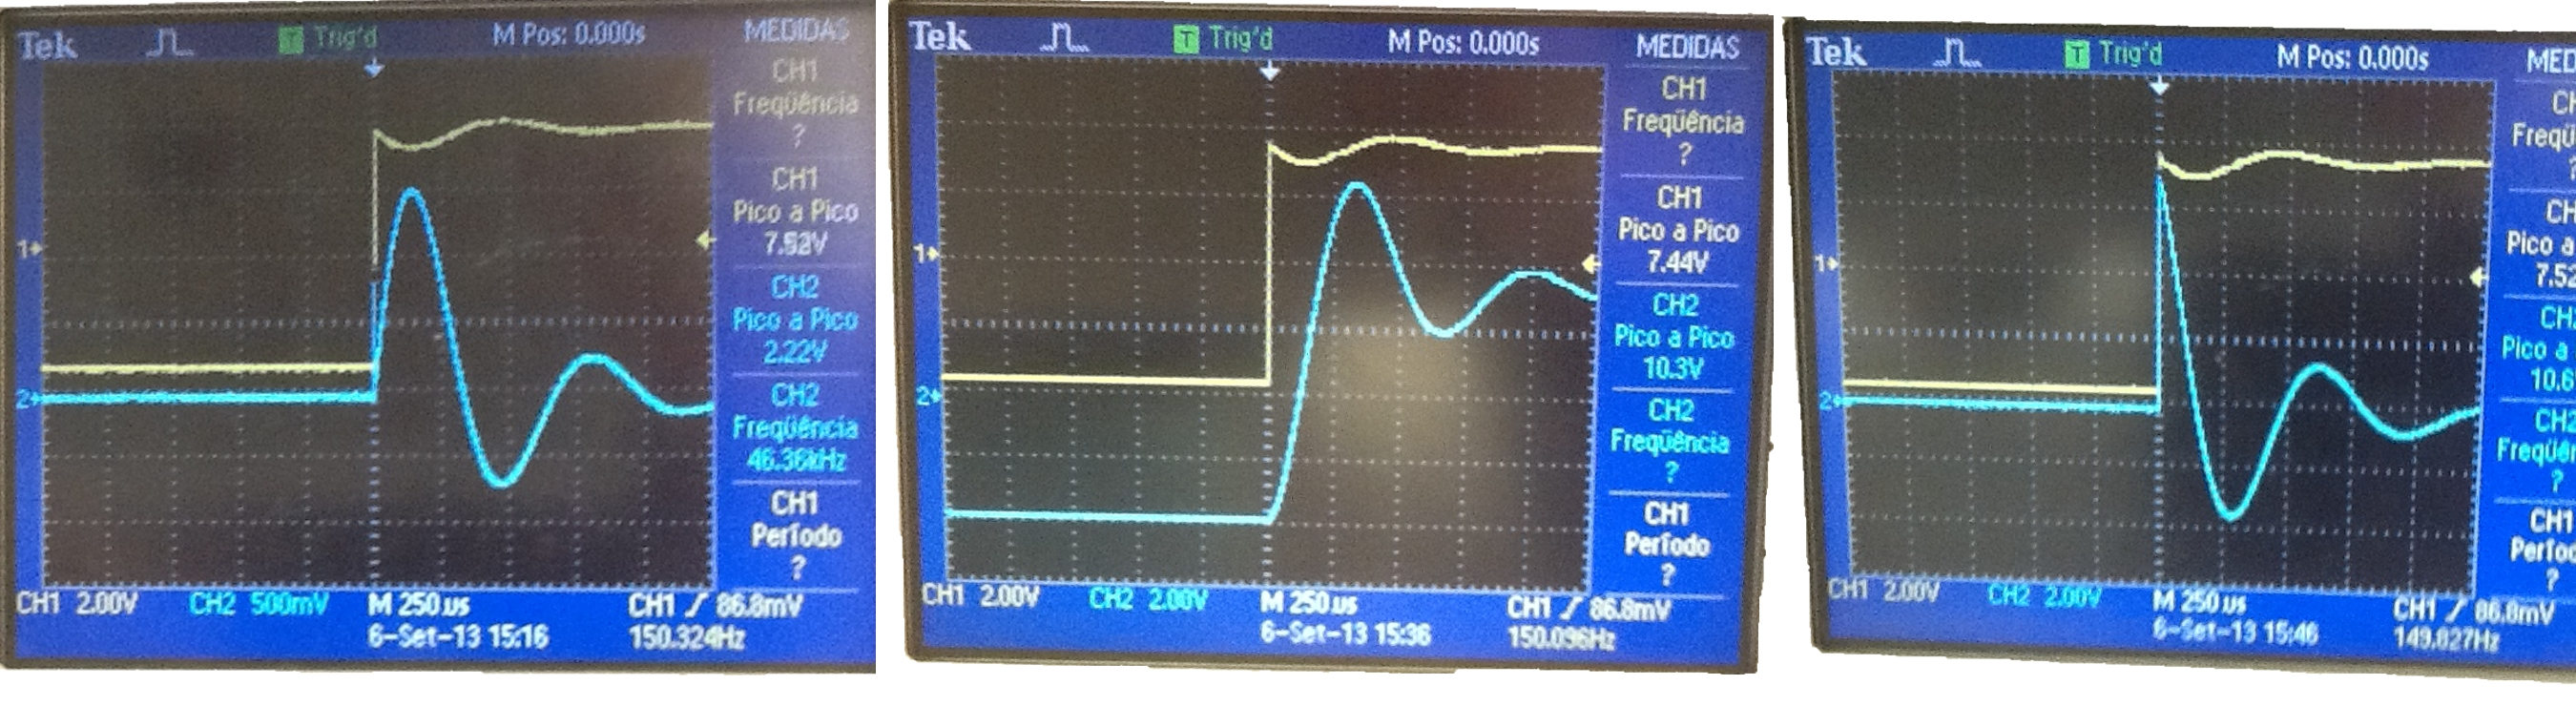
\includegraphics[scale=0.18]{img/mysub.jpg}
  \caption{Resistor, Capacitor e Indutor subamortecidos}
\end{figure}
\\
\\
\\
\\
\\
\\
Como podemos ver, as fotos do experiementais condizem com os gráficos traçados na figura acima.
Agora ao tratarmos o sobre-amortecimento temos a equação o $\omega = j \beta$, j é um imaginário puro onde: $q(t)=C E_{pp}[1 - e^{\frac{-t}{\tau}}(cosh(\beta t)+ \frac{1}{\beta t}sen(\beta t))] (Q < \frac{1}{2}) $ E no caso de amortecimento crítico temos $\omega = 0$ e como solução da equação diferencial temos: $q(t) = C E_{pp}[1 - (1 + \frac{t}{\tau})e^{\frac{-t}{\tau}}] (Q = \frac{1}{2})$\\
Com as cargas definidas temos as voltagens dadas por: $V_c = \frac{q}{C}; V_R = R \frac{dq}{dt} e V_L = L \frac{d^2q}{dt^2}$.\\
Como a tabela abaixo mostra temos o resultado destas 3 equações para os amortecimentos:,
\begin{figure}[!htb]
  \centering
  \label{tabela}
  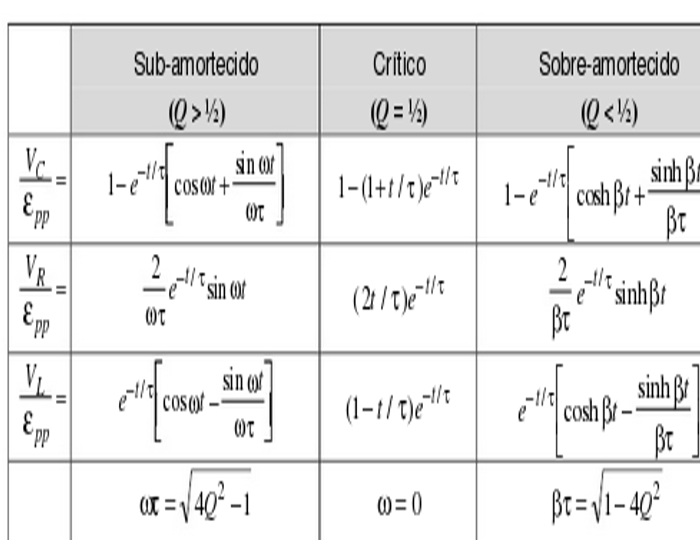
\includegraphics[scale=0.40]{img/tabela.jpg}
  \caption{Equações dos amortecimentos}
\end{figure}
Com isso esperamos os seguintes gráficos para o sobre-amortecimento e o amortecimento crítico, sendo a curva indicada por $Q = 0.3$ e $Q = 0.5$, respectivamente.
\begin{figure}[!htb]
  \centering
  \label{tabela}
  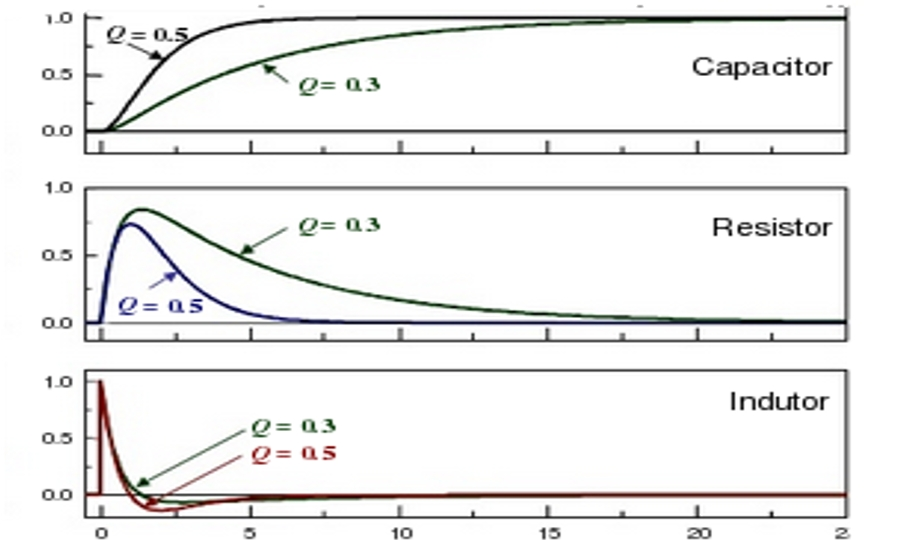
\includegraphics[scale=0.40]{img/qfig.jpg}
  \caption{Sobre-amortecido e amortecimento crítico teóricos}
\end{figure}
E abaixo temos as fotos obtidas em nosso experimento:
\begin{figure}[!htb]
  \centering
  \label{tabela}
  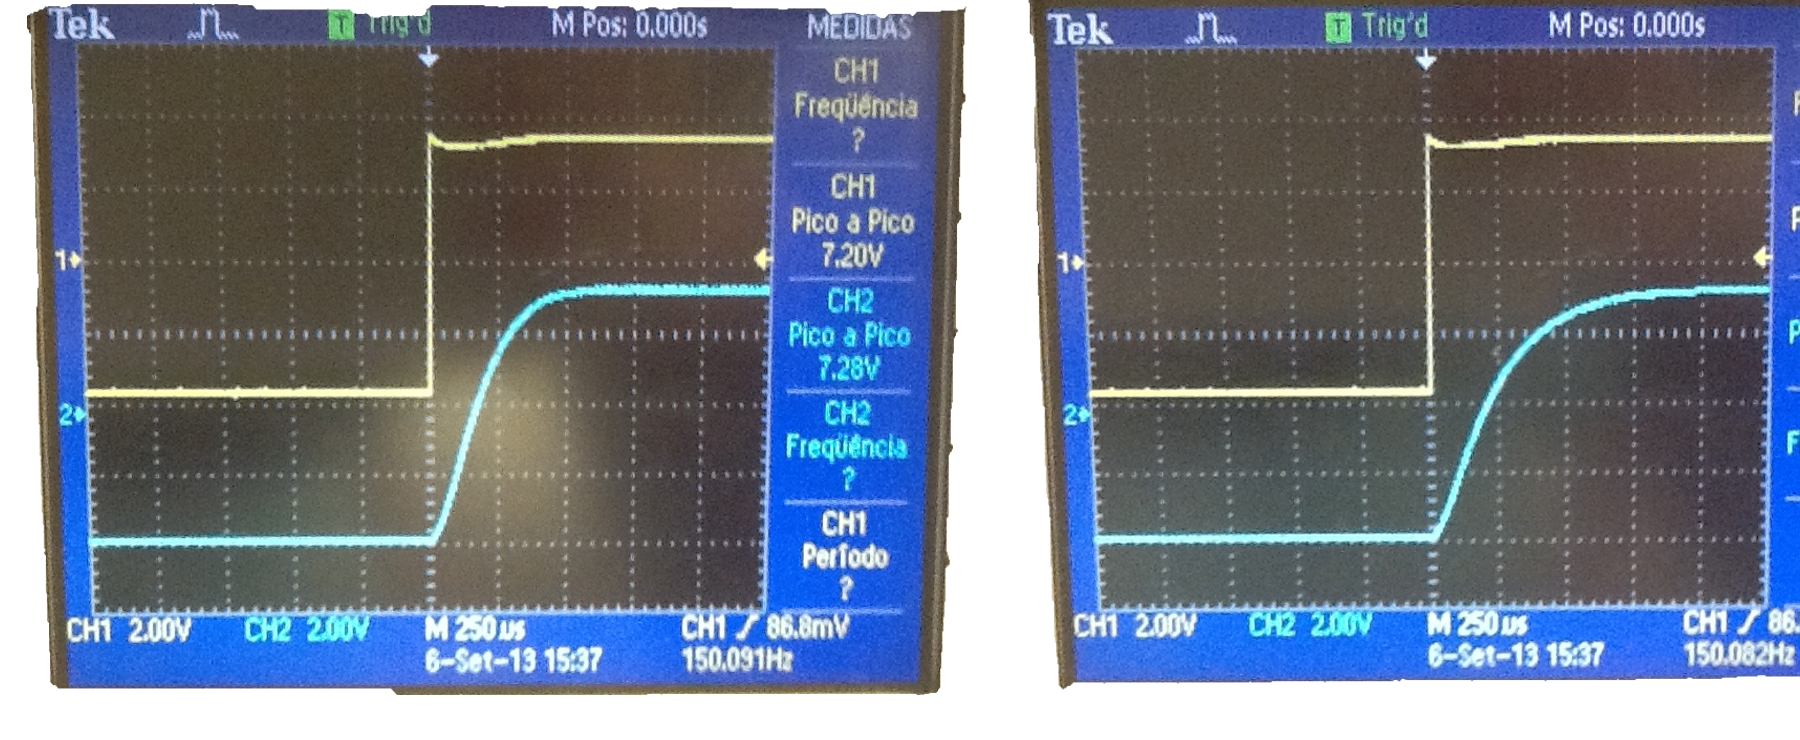
\includegraphics[scale=0.18]{img/rcrit.jpg}
  \caption{Resistor sobre-amortecido e criticamente amortecido}
\end{figure}
\begin{figure}[!htb]
  \centering
  \label{tabela}
  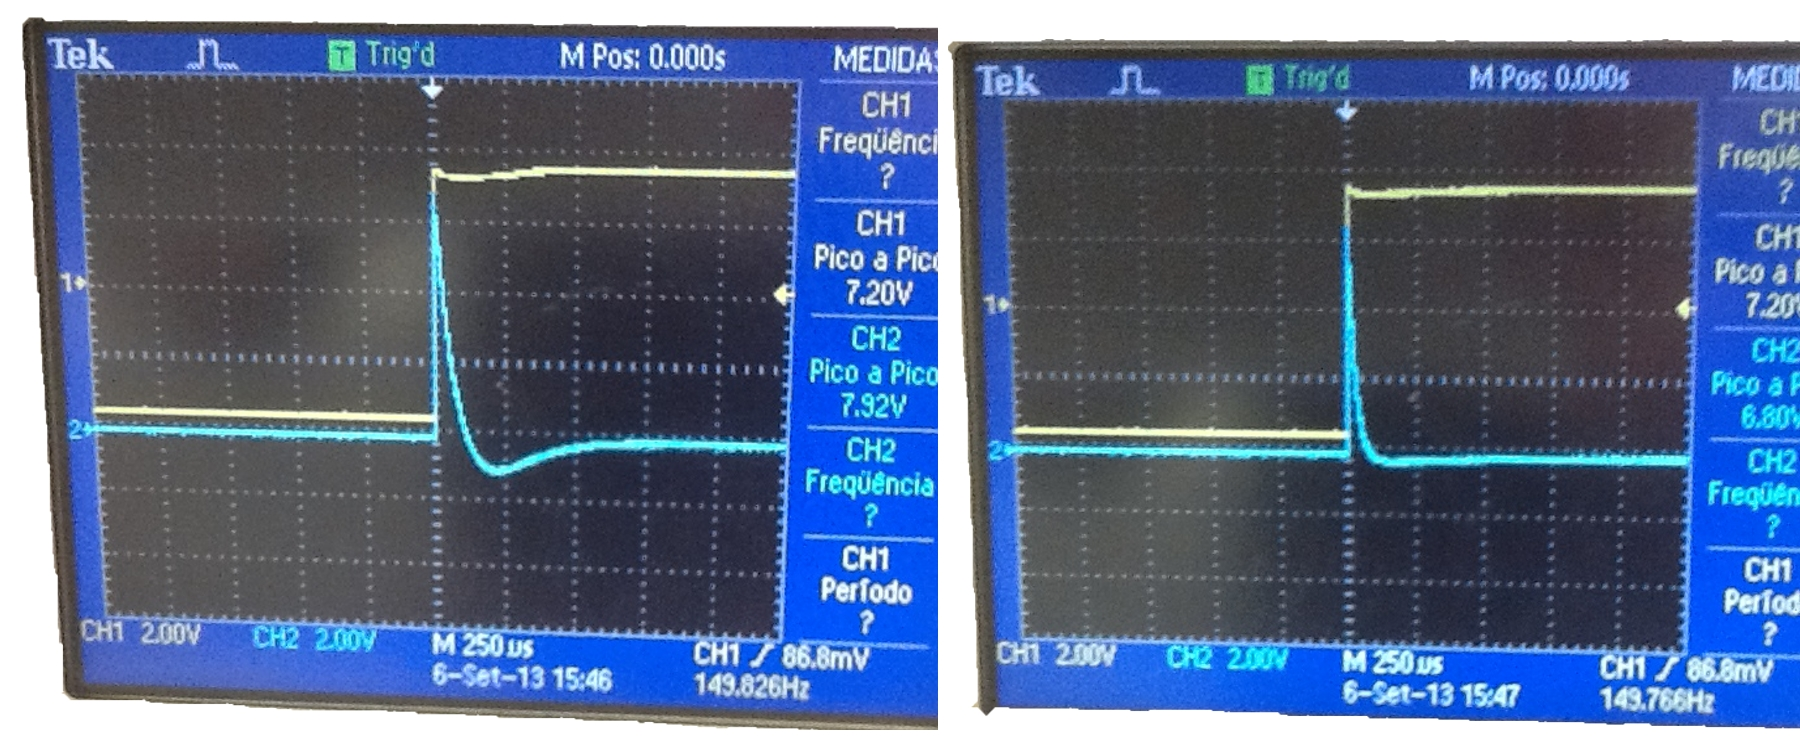
\includegraphics[scale=0.18]{img/indcrit.jpg}
  \caption{Indutor sobre-amortecido e criticamente amortecido}
\end{figure}
Agora, por fim, no experimento, colocamos para resistências pequenas ( da ordem de 10$\Omega$ ) obtemos as seguintes fotos:
\begin{figure}[!htb]
  \centering
  \label{tabela}
  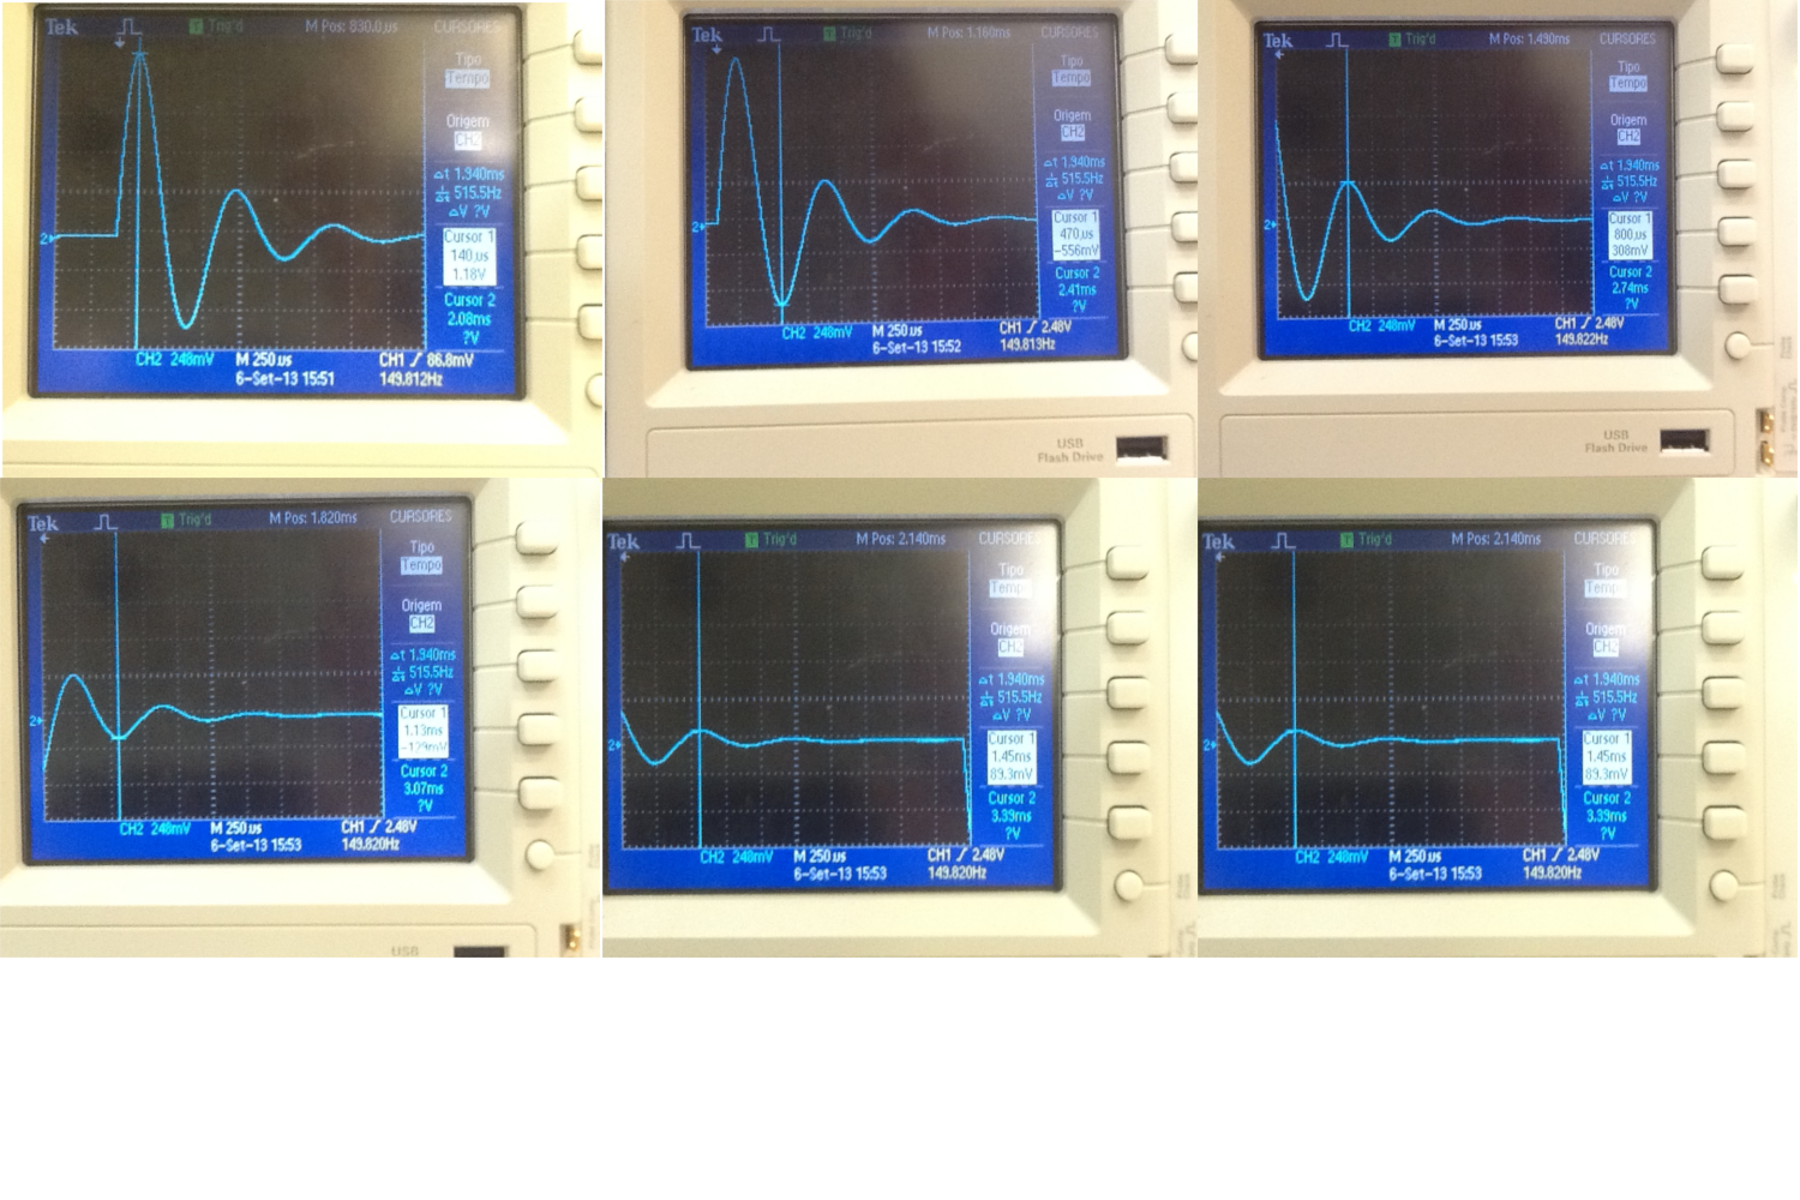
\includegraphics[scale=0.20]{img/a1v.png}
  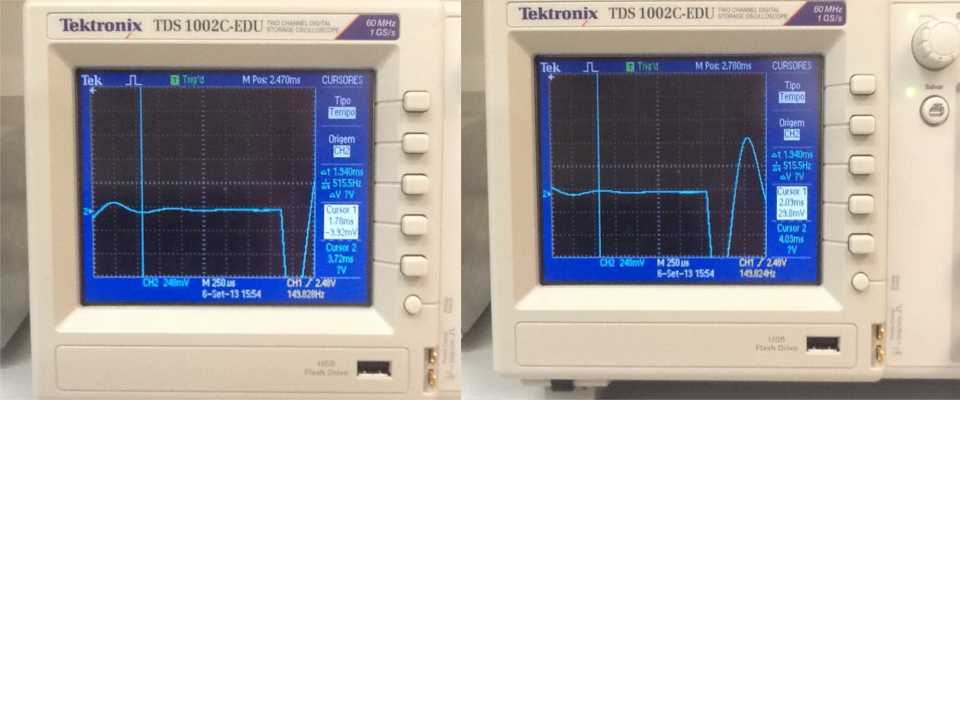
\includegraphics[scale=0.38]{img/a2v.png}
  \caption{Máximos e mínimos locais acima do eixo V}
\end{figure}
\begin{figure}[!htb]
  \centering
  \label{tabela}
  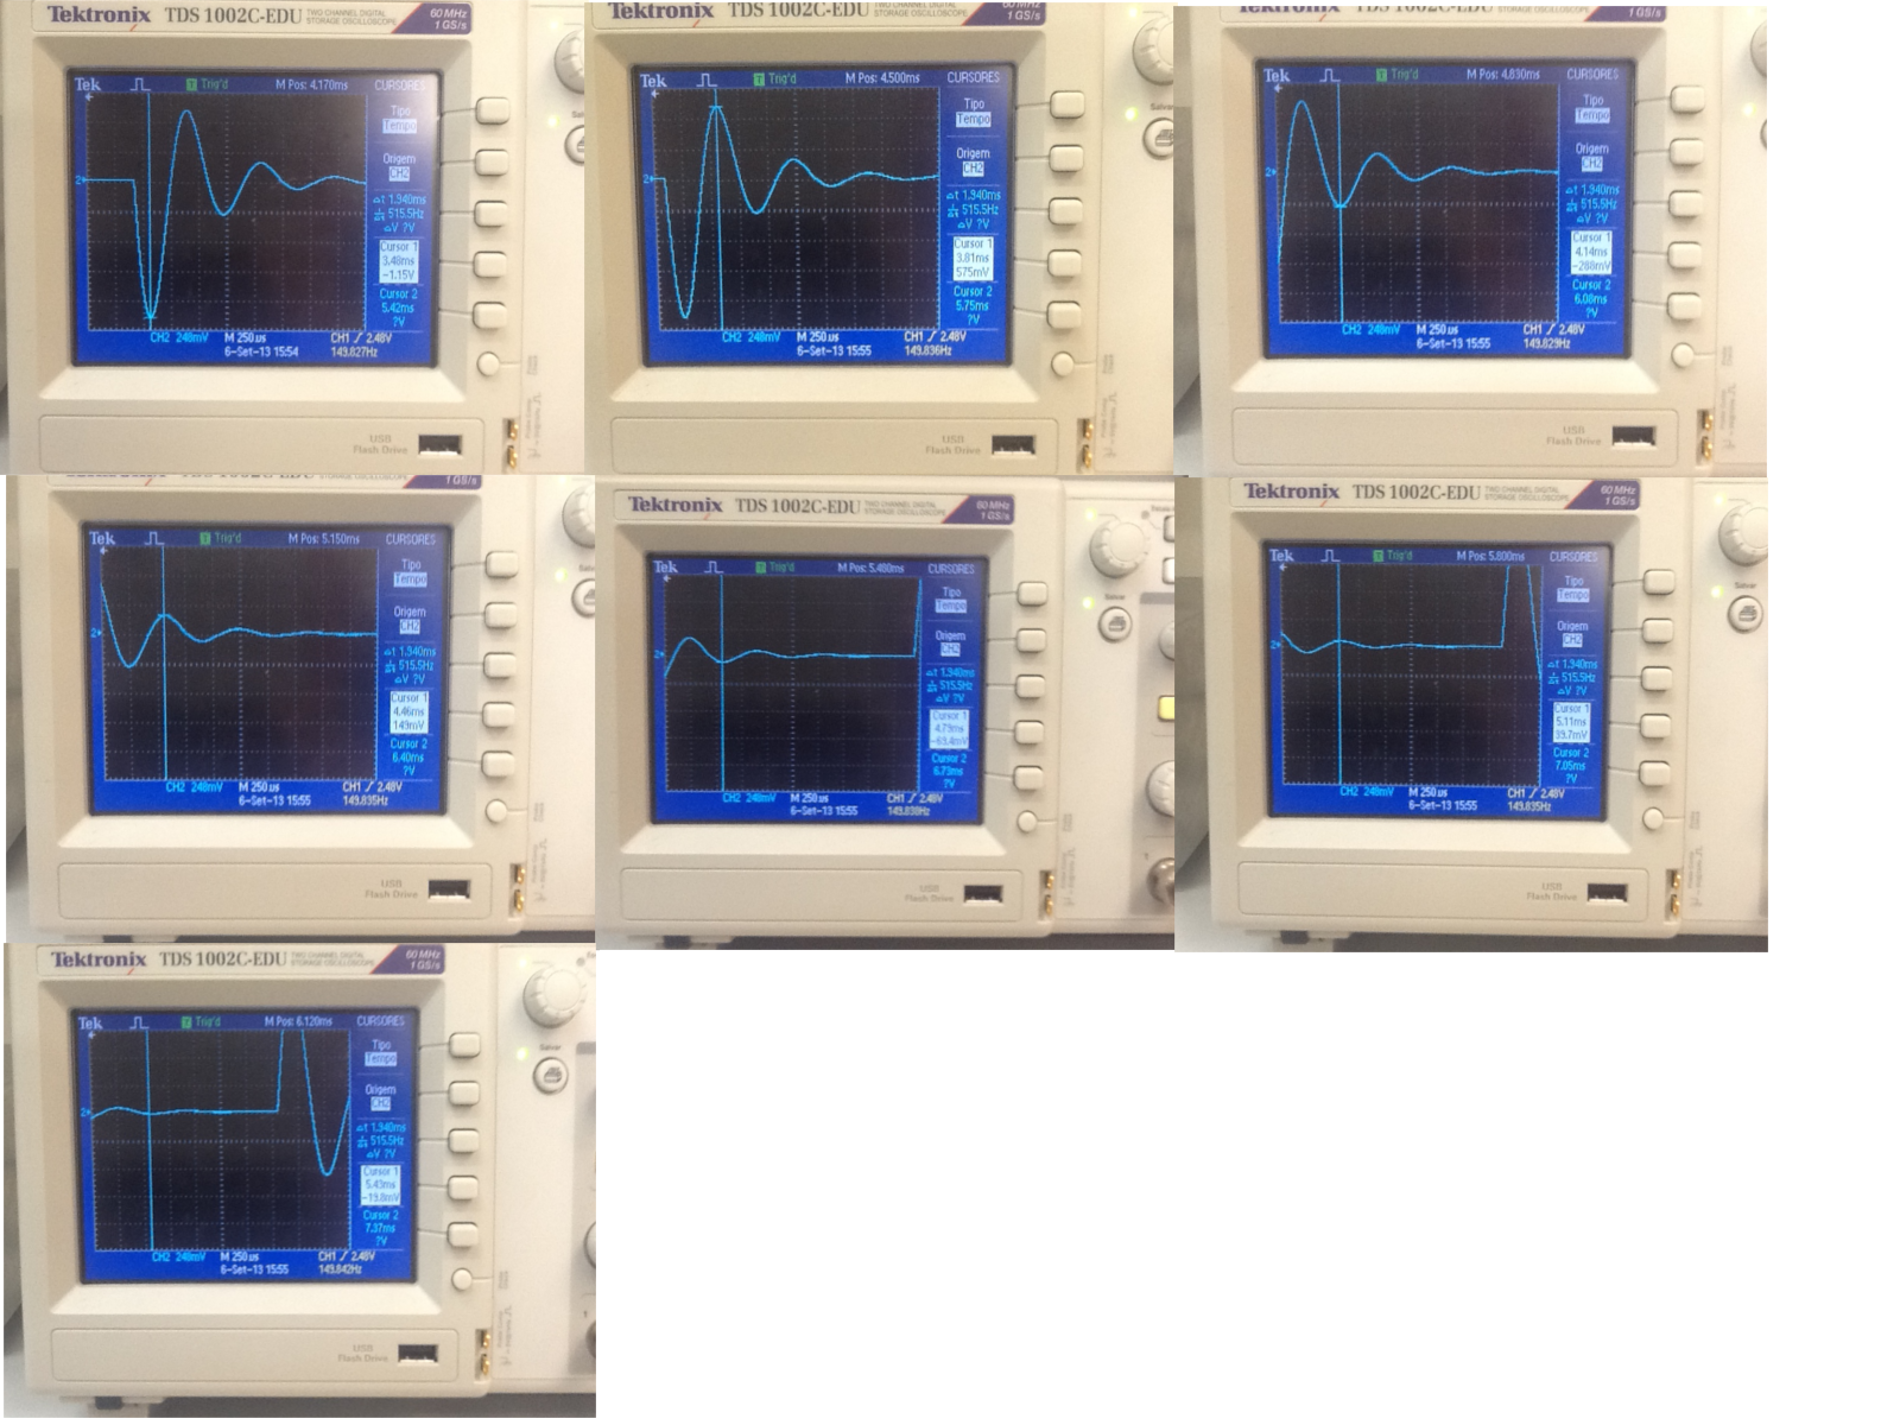
\includegraphics[scale=0.20]{img/abixo.png}
  \caption{Máximos e mínimos locais abaixo do eixo V}
\end{figure}
Podemos ver a amplitude $A_n$ nos máximos e mínimos locais como função do tempo e a frequência de oscilação, $f_n$.
\begin{table}
  \tiny
  \centering
  \begin{tabular}{|c|c|c|c|c|c|c|c|}
    \hline
    $A_n$ & Tempo ($10^{-6}$) & Escala V & Escala T & Erro V & Erro T & Tempo & $ln(A_n)$\\
    \hline
    1.18 & 140 & 248 & 250 & 0.06644 & 0.0000145 & 0.00014 & 0.165514438477573 \\
0.556 & 470 & 248 & 250 & 0.03524 & 0.000031 & 0.00047 & -0.586986984731555 \\
0.308 & 800 &  248 & 250 & 0.02284 & 0.0000475 & 0.0008 & -1.17765549600856 \\
0.129 & 1450 & 248 & 250 & 0.01389 & 0.00008 & 0.00145 & -2.04794287462046\\
0.0893 & 1450 & 248 & 250 & 0.011905 & 0.00008 & 0.00145 & -2.41575379109968\\
0.00992 & 1780 & 248 & 250 & 0.007936 & 0.0000965 & 0.00178 & -4.61320235768536\\
0.00298 & 2090 & 248 & 250 & 0.00893 & 0.000112 & 0.00209 & -3.51324688547078\\
1.15 & 3480 & 248 & 250 & 0.06494 & 0.0001815 & 0.00348 & 0.139761942375159\\
0.575 & 3810 & 248 & 250 & 0.03619 & 0.000198 & 0.00381 & -0.553385238184787\\
0.288 & 4140 & 248 & 250 & 0.02184 & 0.0002145 & 0.00414 & -1.24479479884619\\
0.149 & 4460 & 248 & 250 & 0.01489 & 0.0002305 & 0.00446 & -1.90380897303668\\
0.0694 & 4790 & 248 & 250 & 0.01091 & 0.000247 & 0.00479 & -2.66786841146938\\
0.00511 & 39700 & 248 & 250 & 0.0076955 & 0.0019925 & 0.0397 & -5.27655587476652\\
0.0198 & 5430 & 248 & 250 & 0.00843 & 0.000279 & 0.00543 & -3.92207334128165\\

    
    \hline
  \end{tabular}
  \caption{Tabela de dados (Amplitudo e Tempo)}
\end{table}
\begin{figure}[!htb]
  \centering
  \label{mysub}
  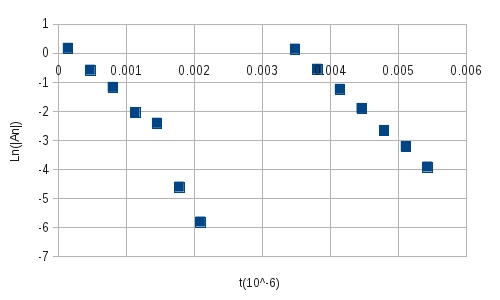
\includegraphics[scale=0.50]{img/g1.jpg}
  \caption{Gráfico Amplitude X Tempo}
\end{figure}
\\
\\
\\
\\
\\
\\
\\
\\
\\

\section{Conclusão}
Conforme observamos nos circuitos RC, obtivemos a resposta esperada para altas frequências em um passa-baixa, ou seja, atuando como um integrador. O mesmo foi observado no circuito diferenciador, sendo para baixas frequências, quando este está sendo alimentado com uma tensão de frequência alta, o mesmo funciona como um \emph{buffer}, ou seguidor de tensão \footnote{no circuito passa-baixa esse efeito é observado para baixas freq.}.
Para o circuito RLC, observamos os casos de amortecimento para diferentes valores na resistência de década (140$\Omega$ e 740$\Omega$), em cada componente do sistema. 
\section{Referências}
\begin{itemize}
\item Sedra Smith, microeletronics circuits 5th edition
\item \url{http://sites.ifi.unicamp.br/f429/files/2011/02/lista1_teorica.pdf} 
\end{itemize}
\end{document}


